\subsection*{The Set of Positive Rational Numbers}
If we expect to find an uncountable set in our usual number systems, the rational numbers might be the place to start looking.  One of the main differences between the set of rational numbers and the integers is that given any integer $m$, there is a next integer, namely $m + 1$.  This is not true for the set of rational numbers.  We know that $\Q$ is closed under division (by nonzero rational numbers) and we will see that this property implies that given any two rational numbers, we can also find a rational number between them.  In fact, between any two rational numbers, we can find infinitely many rational numbers.  It is this property that may lead us to believe that there are ``more'' rational numbers than there are integers.

The basic idea will be to ``go half way'' between two rational numbers.  For example, if we use $a = \dfrac{1}{3}$ and $b = \dfrac{1}{2}$, we can use
\[
\frac{a+b}{2} = \frac{1}{2} \left( \frac{1}{3} + \frac{1}{2} \right) = \frac{5}{12}
\]
as a rational number between $a$ and $b$.  We can then repeat this process to find a rational number between 
$\dfrac{5}{12}$ and $\dfrac{1}{2}$.

So we will now let $a$ and $b$ be any two rational numbers with $a < b$ and let $c_1 = \dfrac{a+b}{2}$.  We then see that%
\label{tworationals}%
\begin{align*}
c_1 - a &= \frac{a+b}{2} - a &  b- c_1 &= b - \frac{a+b}{2} \\
        &= \frac{a+b}{2} - \frac{2a}{2} &  &= \frac{2b}{2} - \frac{a+b}{2} \\
        &= \frac{b-a}{2}                &  &= \frac{b-a}{2}
\end{align*}
Since $b > a$, we see that $b - a > 0$ and so the previous equations show that $c_1 - a > 0$ and $b - c_1 > 0$.  We can then conclude that $a < c_1 < b$.

We can now repeat this process by using $c_2 = \dfrac{c_1 + b}{2}$ and proving that $c_1 < c_2 < b$.  In fact, for each natural number, we can define
\[
c_{k + 1} = \frac{c_k + b}{2}
\]
and obtain the result that $a < c_1 < c_2 < \cdots < c_n < \cdots < b$ and this proves that the set 
$\left\{ c_k \mid k \in \mathbb{N} \right\}$ is a countably infinite set where each element is a rational number between $a$ and $b$.  (A formal proof can be completed using mathematical induction.)  See Exercise~(\ref{exer:tworationals}).

This result is true no matter how close together $a$ and $b$ are.  For example, we can now conclude that there are infinitely many rational numbers between 0 and $\dfrac{1}{10000}$.  This might suggest that the set $\mathbb{Q}$ of rational numbers is uncountable.  Surprisingly, this is not the case.  We start with a proof that the set of positive rational numbers is countable.

\begin{theorem}\label{T:positiverationals}
The set of positive rational numbers is countably infinite.
\end{theorem}
%
\begin{myproof}
We can write all the positive rational numbers in a two-dimensional array as shown in 
Figure~\ref{fig:positiverationals}.
%
\begin{figure}[h]
\begin{center}
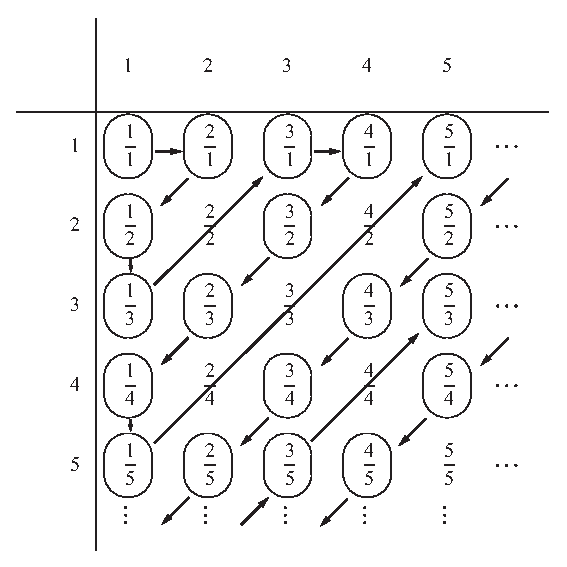
\includegraphics{figps-rationals.eps}
\caption{Counting the Positive Rational Numbers}\label{fig:positiverationals}
\end{center}
\end{figure}
The top row in Figure~\ref{fig:positiverationals} represents the numerator of the rational number, and the left column represents the denominator.  We follow the arrows in 
Figure~\ref{fig:positiverationals} to define $f\x \mathbb{N} \to \mathbb{Q}^+$.  The idea is to start in the upper left corner of the table and move to successive diagonals  as follows:
\begin{itemize}
\item We start with all fractions in which the sum of the numerator and denominator is 2 
$\left( \text{only } \dfrac{1}{1} \right)$.  So $f ( 1 ) = \dfrac{1}{1}$.

\item We next use those fractions in which the sum of the numerator and denominator is 3.  So 
$f ( 2 ) = \dfrac{2}{1}$ and $f ( 3 ) = \dfrac{1}{2}$.

\item We next use those fractions in which the sum of the numerator and denominator is 4.  So 
$f ( 4 ) = \dfrac{1}{3}$, $f ( 5 ) = \dfrac{3}{1}$.  We skipped 
$\dfrac{2}{2}$ since $\dfrac{2}{2} = \dfrac{1}{1}$.  In this way, we will ensure that the function $f$ is a one-to-one function.
\end{itemize}
We now continue with successive diagonals omitting fractions that are not in lowest terms.  This process guarantees that the function $f$ will be an injection and a surjection.  Therefore, 
$\mathbb{N} \approx \mathbb{Q}^+$ and $\text{card} ( \mathbb{Q}^+ ) = \aleph_0$.
\end{myproof}

\newpar
\note For another proof of Theorem~\ref{T:positiverationals}, see exercise~(\ref{A:Qcountable}) on page~\pageref{A:Qcountable}.

\newpar
Since $\mathbb{Q}^+$ is countable, it seems reasonable to expect that $Q$ is countable.  We will explore this soon.  On the other hand, at this point, it may also seem reasonable to ask, 
\begin{center}
``Are there any uncountable sets?''
\end{center}
The answer to this question is yes, but we will wait until the next section to prove that certain sets are uncountable.  We still have a few more issues to deal with concerning countable sets.
\endinput
